\section{Implementation and workflow}\label{sec:Implementation}


\subsection{\textbf{Dependencies}}
The package \textit{OnlineFileSelector} resides in the \textit{Online} project. Furthermore it uses the following packages : \textit{Event/DAQEvent}, \textit{DAQ/MDF}, \textit{LCG\_Interfaces/sqlite} and \textit{LCG\_Interfaces/AIDA}.

\subsection{\textbf{Workflow}}
The ApplicationManager initializes the required services (for details see ADD \cite{mato1998gaudi}), among them the \textit{Poller} and the \textit{EventSelector}.\par

\subsubsection{\textbf{Poller}}
The initialization is completed by calling the \textit{initialize()} method of the poller, which first connects to the database where it will store the run-related information (or creates a new database if one does not exist). The execution continues with the \textit{start()} method, which sets the timer and starts the countdown until the next polling.\par
When the timer expires, the \textit{timerHandler()} method gets called. It will first call the \textit{poller()} method which takes as argument the directory to be scanned for new files. Then it will start distributing the file paths to the EventSelector and it will stop either when the listener has been served or when there are no more files to distribute.The process for distributing the files is as follows:~First the file path is removed (\textit{remFromfileNames()}) from the list of available file paths, which was filled during the last polling period.From that path we extract the run number (\textit{getRunFileNumber()}) which we will use to check:\par
\begin{itemize}
\item if we had tried to open it but we encountered an error and the file should not be tried again (\textit{isDefect()}),\par
\item if we have already opened it and is currently being processed (\textit{isBookKept()}), or\par
\item if the file has already been processed (\textit{isProcessed()})\par
\end{itemize}
 The run extraction method takes as argument a regular expression to match with the run number. If one of the above mentioned cases occurs we skip the processing of the current run, otherwise we pass the file path on to the listener,which is then removed from the waiting spot.\par
Regarding the removal of the listener there are three cases :
\begin{itemize}
\item the communication between the \textit{Poller} and the \textit{EventSelector} takes place (either successful opening of the received file or not) and then the listener is removed (from inside \textit{alertSvc()})\par
\item the listener does not manage to acquire the waiting lock before going idle -erroneous behaviour, removed from the list from inside \textit{goIdle()}\par
\item the listener fails for some reason. To cover this case there is a removal taking place inside \textit{timerHandler()}, after the delivery of the file. In normal cases the listener will have been already removed from \textit{alertSvc()}\par
\end{itemize}
When the distribution of the files is over, we empty the vector holding the remaining file paths (if any) and the timer is reset.\par
At the end of the execution cycle, the \textit{stop()} method is called which stops the service and the countdown of the timer. It is followed by a call to the \textit{finalize()} closes the connection to the file database.\par

\begin{figure}

\caption{\textit{The function of the polling service}}
\centering
\fbox{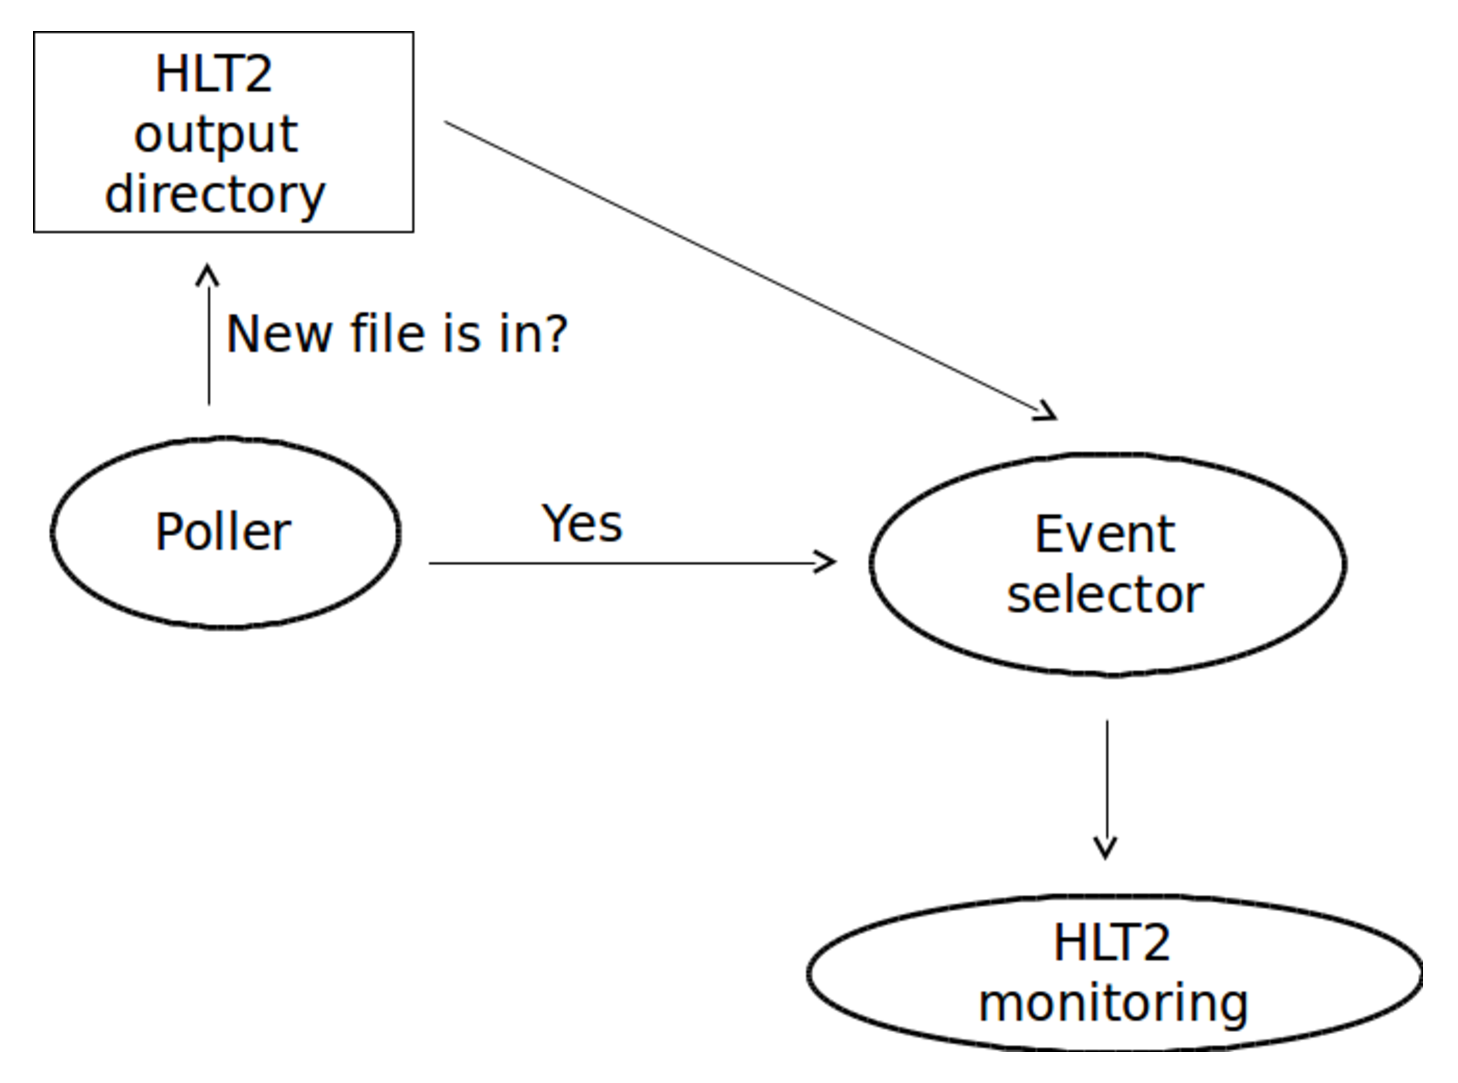
\includegraphics[height=\textheight,width=.8\textwidth, keepaspectratio=true]{figs/poller}}\par

\end{figure}


\subsubsection{\textbf{EventSelector}}
In the initialization of the \textit{EventSelector} pointers to other services are acquired. What we need to add to an \textit{EventSelector} to make it possible for it to use the poller are the following services, for which we acquire the necessary pointers : \textit{FilePoller}, \textit{HistogramDataSvc}, \textit{RootHistSvc} and \textit{HistogramPersistencySvc}. For details on the functionality of the latter three see \cite{mato1998gaudi}. Then we create the lock that will control the waiting/resuming of the \textit{EventSelector} during its interaction with the poller, and we initialize its value to zero, which means that at the beginning of its execution the \textit{EventSelector} will wait for input from the poller. Finally we initialize the counter \textit{m\_evtCount}, which counts the events read from a file and helps in deciding when the \textit{EventSelector} will go idle.
The \textit{start()}/\textit{stop()} methods are inherited from the base class \textit{Service}.\par
The \textit{EventLoopMgr} will use the \textit{EventSelector} to acquire the next event for processing -the \textit{next()} method of the \textit{EventSelector} gets called. After two initial checks regarding saving the histograms and updating the database (see later), the \textit{EventSelector} will check whether there is an input context (\textit{pCtxt != 0}).
If there is not, the \textit{EventSelector} will return StatusCode::FAILURE.\par
If there is an input context, we first have to check if this is the first connection (meaning \textit{m\_firstConnection == 0}) to an input file that the \textit{EventSelector} is trying to establish. Without this check we cannot safely call the \textit{receiveData()} method to read the next event.\par

\begin{itemize}
\item If it is the first connection the \textit{EventSelector} will finally go idle, that is it will connect to \textit{poller} and wait for an input file path (by calling the \textit{goIdle()} method).\par
\item If it is not the first connection, the \textit{EventSelector} will call \textit{receiveData()} to read the next event; if the call is successful the \textit{EventSelector} will increase the corresponding event counters and return StatusCode::SUCCESS. If it cannot read the next event (e.g. because there are no more events in the file), the \textit{EventSelector} will go idle after updating the database with the number of events it has read from the last input file and saving the histogram sets.\par
\end{itemize}
For the next calls of the  \textit{next()} method there are two checks preceding the input context check.\par
The first \textit{m\_maxNoEvt == m\_evtCount} checks whether we have reached the maximum number of events we want to read from one file. If we have, then the \textit{EventSelector} updates the database with the number of events so far read, resets the event counter, saves the histograms and then goes idle, waiting for the next file.If we want to read until the end of the file, we should set the \textit{m\_maxNoEvt} to -1.\par
%The second \textit{m\_EvtHisto} $\leq$  \textit{m\_totalEvt} checks whether we have read the necessary number of events to make a set of histograms. If yes, the event counter is reset to start counting again for the next set, we save the current set by calling \textit{saveHistos()} and then the \textit{EventSelector} goes idle.ONLY NEEDED IF WE WANT MORE THAN ONE HISTOFILES FROM THE SAME RUN\par
The second \textit{m\_runNum} $\neq$ \textit{m\_prevRun} checks whether the run has changed. If yes, it resets the event counter and changes the name of the file which will contain the next set of histograms.Then the \textit{EventSelector} continues reading events from the new file (and thus run). This check covers the case where the minimum number of events to produce a set of histograms is bigger then the events we have read from a file before changing it (e.g. covers the case of a very small run).\par
After having gone idle, the \textit{EventSelector} will wait at the corresponding lock (\textit{m\_suspendLock}) until the poller serves it with a file. In order for this to happen, the poller will call the \textit{alertSvc()} method of the \textit{EventSelector} passing as argument the file path to read from. This method before exiting will change the value of the \textit{m\_firstConnection} to 1, to signal that there has been at least one connection established.Next, it will get the current input context and update it with the new file path by calling \textit{resetCriteria()}.If the context update is successful, the \textit{EventSelector} reports back to the poller the \textit{successful opening} of the new file using \textit{statusReport()}. This means that the file and run will be added to the file database with a status flag of 0 : the file has been opened but we have not finished processing it.Then the poller will remove the \textit{EventSelector} from the waiting spot, extract the new run number from the file path and generate accordingly the new histogram set name.It will finally resume the operation of the \textit{EventSelector}, which will continue from the point where the last call of \textit{goIdle()} was made.\par
At the end of the execution cycle, the inherited \textit{stop()} method is called and then the \textit{finalize()}. In the \textit{finalize()} method we reset the counters, remove the acquired interfaces by setting the pointers to them to 0 and we delete the wait/resume lock of the \textit{EventSelector}.

\subsubsection{\textbf{Details about Poller methods and member variables}}

\begin{itemize}

\item std::string m\_scanDirectory : this is the directory that the poller will check periodically for files, which will then distribute to the listeners\par
\item int m\_alrmTime : the time interval between two successive pollings\par
\item std::deque$<$std:string$>$ m\_fileNames : the list of the file paths that were found in the scanned directory during the last polling.\par 
\bigskip\noindent
The \textit{std::deque} container was chosen for the above list as it implements a First In First Out structure, which is what we want especially for the listeners : the poller should serve first the listener who asked first for a new file. Furthermore, a  \textit{std::deque} performs better than a vector at the removal of its first element and grows more efficiently in size.\par
\bigskip\noindent
\item mutable $<$IAlertSvc*$>$ m\_EvtSelector : the listener waiting for input from the poller. It is kept in the form of a pointer to its \textit{IAlertSvc} interface.\par
\item sqlite3* m\_FileInfo : the handler of the database keeping the file/run information.\par
\bigskip\noindent
The necessary accesor methods for the above private member variables are provided : \textit{addTofileNames,remFromfileNames}.\par
Some more implementation details about methods that were mentioned in the workflow:\par
\item StatusCode poller(const std::string scan\_path) : This is the method that performs the polling.It uses \textit{readdir\_r} to scan the directory. If it finds a file, it adds it to the file list whereas if it finds another directory it calls itself recursively to scan it (apart from the current (\textit{\"~.\"}) and previous  (\textit{\"~..\"}) directories).\par
\item StatusCode statusReport(StatusCode status,const std::string file) : This method gives feedback to the poller about the \textit{opening} of the file from the \textit{EventSelector}.If the opening was unsuccessful the method \textit{issueAlarm()} is called, which inserts an error record into the database containing the file name, the run number and the value of -1 in the event counter and status flag.If the opening was succesful, we insert the file name into the database, marking it as unprocessed/currently in process (\textit{StatusFlag == 0}), using the method \textit{markBookKept()}.\par
\item const StatusCode issueAlarm(const std::string& msg) : In case the \textit{EventSelector} does not manage to open a file from the path it has received, it is not enough to print a message reporting it. This method provides support for this case by adding an entry in the database with the name of the file that failed to be opened, the run it belongs to and the value of -1 in the \textit{StatusFlag} and '\textit{TotalEvents} fields.\par
\item StatusCode isBookKept(const std::string file) : It checks if the file passed as its argument is in the database with \textit{StatusFlag == 0},i.e. it is currently being processed.\par
\item StatusCode isProcessed(const std::string file) : It checks if the file passed as its argument is in the database with \textit{StatusFlag == 1}.\par
\item StatusCode updateStatus(const std::string file, int events) : It updates the record in the database which corresponds to the file passed as argument, with the number of events passed as the second argument.\par

\end{itemize}


\subsubsection{\textbf{Details about EventSelector methods and member variables}}
\begin{itemize}
\item std::string m\_HistoDirectory : this is the output directory for the histogram sets saved by the poller\par
\item StatusCode goIdle() const : This method is called for the transition of the \textit{EventSelector} from a running to an idle state.It first sets the \textit{m\_isWaiting} flag to true. Then the \textit{EventSelector} is added to the listener spot of the poller by calling \textit{addListener()}.If the registration to the poller is successful, the \textit{EventSelector} waits at the \textit{m\_suspendLock}. If it cannot acquire the waiting lock it removes itself from the listener spot by calling \textit{remListener()}. Either after its removal or when it resumes execution after having successfully waited, the \textit{m\_isWaiting} flag is set to false.\par

\item StatusCode saveHistos() const : This method is responsible for saving the histogram sets. Normally these steps would be carried out when the event loop would have finished, but since the poller will be constantly running this will happen only at the end of the processing of all runs. The need to save the sets at the end of each run called for the integration of this code here. The histograms are traversed, conversed to their permanent representation (e.g. ROOT) and saved. In order to create a new file for each saveset and not overwrite the same saveset again and again, the histograms must be reset and a new file name has to be selected for the histogram file. Whenever we have to save the histograms (that is either when we have reached the necessary number of events or when the run has changed), the conversion service (\textit{m\_RootHistSvc}) is stopped and finalised. The methods \textit{sysStop()} and \textit{sysFinalize()} are called instead of the  \textit{stop()} and \textit{finalize()} to avoid execution errors because these methods change the state of the machine according to their function from running to configure.If a new file is going to be opened next, that is if a new run is going to be processed, the name of the histogram file is changed. It is in this method (\textit{setNewHistosName()}) that we reintialize and restart the conversion service.


\end{itemize}


%\section{How to run and test Poller}\label{sec:HowTo}
%\subsection{\textbf{Prerequisites}}
%This section will give some instructions on how to run the polling service. It takes for granted that the \textit{EventSelector} used will have been modified to use the poller, as described above.\par
%The \textit{OnlineFileSelector} package should be in the same \textit{VanDerMeer} project directory, or the monitoring scripts should be able to "see" it by including it in the \textit{requirements} file of their \textit{cmt} directory.\par.\subsection{\textbf{Running}}
%In order to run the \textit{poller}, an instance of it and of a modified \textit{EventSelector} should be instantiated and its variables initialized (scan directory, alarm timer). Next follow the code excerpts of a testing python script that do the job : \par

%\begin{itemize}
%\item Import : from Configurables import ( \par
%             \hspace{20mm} LHCb\_MDFOnlineEvtSelector,\par
%             \hspace{20mm} LHCb\_FilePoller,\par
%                           )  \par
%\item Initial output file : HistogramPersistencySvc().OutputFile = "testPol.root" \par
%\item Poller instantiation and setting parameters : \par
%                 \hspace{20mm}poller = LHCb\_FilePoller('Poller')\par
%                 \hspace{20mm}appMgr.ExtSvc.append(poller)\par
%                 \hspace{19mm}poller.scanDirectory = "/daqarea/lhcb/data/2014/RAW/FULL/LHCb1/TEST"  \par
%                 \hspace{20mm}poller.alarmTime = 3\par
%                 \hspace{20mm}poller.DbName = "./OnlineFileProcessing.db"\par

%\item EventSelector instantiation and setting parameters : \par
%               \hspace{17mm}selector = LHCb\_MDFOnlineEvtSelector('EventSelector')\par
%               \hspace{20mm}appMgr.ExtSvc.append(selector)\par
%               \hspace{20mm}selector.MaxNoEvents = 50000;\par
%               \hspace{20mm}selector.PrintFreq = 10000\par
%               \hspace{20mm}selector.HistogramFile = "testPollerPr.root"\par
%               \hspace{20mm}selector.EvtsForHist = 30000 \par
%               \hspace{20mm}selector.SaveHistoDir = "./HLT2/" \par

%\end{itemize}

%Next follows a typical python script running the poller and producing the same histograms as \textit{HltMassMonitor} program.The histograms will be saved in thedirectory specified in the script.The following procedure should be executed to run the script (provided the following packages are inside \textit{VanDerMeer v6r1}:\textit{OnlineFileSelector, Monitor/HltMonitor, Monitor/CommonMonitor} ):
%\begin{itemize}
%\item run the \textit{SetupVanDerMeer\_v6r1.sh} script, which is inside \textit{Monitor/CommonMonitor/job/}
%\item compile the \textit{OnlineFileSelector} package by running \textit{cmt make} in the \textit{cmt} directory of the package \textit{OnlineFileSelector}
%\item execute (\textit{source}) the setup script in the \textit{cmt} directory of \textit{HltMonitor}
%\item compile the \textit{HltMonitor} by running \textit{cmt make} in its \textit{cmt} directory
%\item run \textit{gaudirun.py testPoller.py} inside \textit{HltMonitor/scripts/}

%\end{itemize}

%\begin{figure}
%\caption{\textit{Sample script}}
%\centering
%\fbox{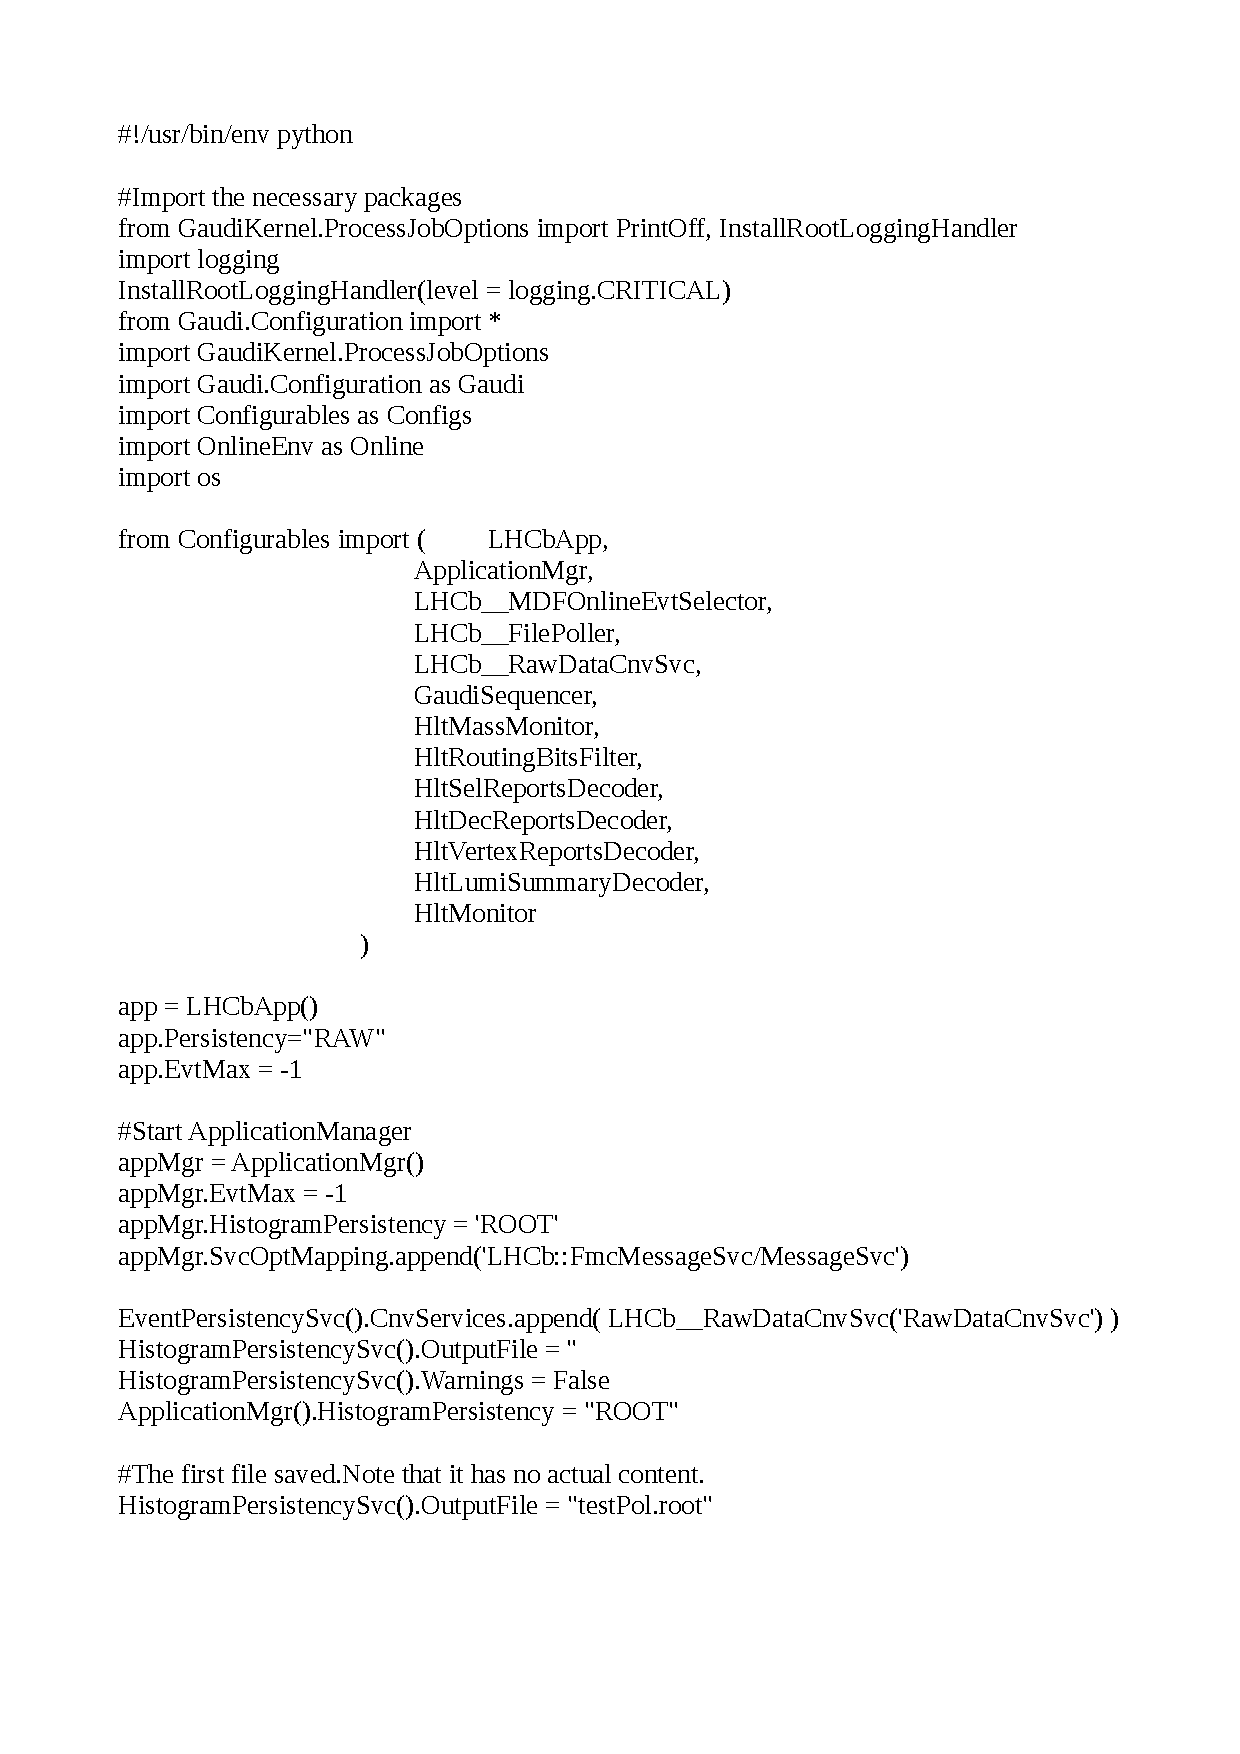
\includegraphics[height=\textheight,width=\textwidth, keepaspectratio=true]{figs/testpoller2}}\par
%\end{figure}\par

%\begin{figure}
%\caption{\textit{Sample script}}
%\centering
%\fbox{\includegraphics[height=\textheight,width=\textwidth, keepaspectratio=true,page=2]{figs/testpoller2}}\par
%\end{figure}\par

%\begin{figure}
%\caption{\textit{Sample script}}
%\centering
%\fbox{\includegraphics[height=\textheight,width=\textwidth, keepaspectratio=true,page=3]{figs/testpoller2}}\par
%\end{figure}\par
